% ══════════════════════════════════════════════════════════════════════════════
%  DQN Self-Play × PER α-Ablation — презентация 10 мин.
%  Минималистичный дизайн, пастельная палитра, 10 слайдов.
%  Build: pdflatex presentation.tex  (дважды)
% ══════════════════════════════════════════════════════════════════════════════
\documentclass[12pt,aspectratio=169]{beamer}

% ── Encoding & Language ───────────────────────────────────────────────────────
\usepackage[utf8]{inputenc}
\usepackage[T2A]{fontenc}
\usepackage[english,russian]{babel}

% ── Math & Graphics ───────────────────────────────────────────────────────────
\usepackage{amsmath,amssymb}
\usepackage{graphicx}
\usepackage{booktabs}
\usepackage{xcolor}
\usepackage{tikz}
\usetikzlibrary{arrows.meta,positioning,backgrounds,calc}

% ── Speaker notes (раскомментировать для двух экранов) ────────────────────────
\usepackage{pgfpages}
% \setbeameroption{show notes on second screen=right}

% ── Пастельная палитра ────────────────────────────────────────────────────────
\definecolor{pdark}{HTML}{2B2D42}        % почти чёрный — основной текст
\definecolor{pblue}{HTML}{6889BB}        % стальной синий — акцент
\definecolor{pteal}{HTML}{52A89E}        % бирюзовый
\definecolor{pgreen}{HTML}{6BAE78}       % мятный зелёный
\definecolor{psalmon}{HTML}{D97A70}      % коралловый
\definecolor{plilac}{HTML}{8F7FBC}       % лиловый
\definecolor{pgray}{HTML}{9AA5B8}        % серый
\definecolor{plbg}{HTML}{EDF1F7}         % светло-голубой фон
\definecolor{pwhite}{HTML}{FFFFFF}

% ── Базовая тема ──────────────────────────────────────────────────────────────
\usetheme{default}
\setbeamertemplate{navigation symbols}{}
\setbeamercolor{background canvas}{bg=pwhite}
\setbeamercolor{normal text}{fg=pdark}
\setbeamercolor{frametitle}{fg=pdark,bg=pwhite}
\setbeamercolor{alerted text}{fg=psalmon}
\setbeamerfont{frametitle}{series=\bfseries,size=\large}
\setbeamerfont{normal text}{size=\normalsize}

% Заголовок слайда — с тонкой линией снизу
\setbeamertemplate{frametitle}{%
  \vspace{0.55em}%
  \insertframetitle\par%
  \vspace{0.12em}%
  {\color{pblue!50}\rule{\textwidth}{0.6pt}}%
  \vspace{0.25em}%
}

% Минимальный футер — только номер
\setbeamertemplate{footline}{%
  \hfill%
  {\color{pgray}\scriptsize\insertframenumber\,/\,\inserttotalframenumber}%
  \hspace{1em}\vspace{0.55em}%
}

% Маркеры списка
\setbeamertemplate{itemize item}{\textcolor{pblue}{\small$\bullet$}}
\setbeamertemplate{itemize subitem}{\textcolor{pteal}{\footnotesize$\circ$}}
\setbeamertemplate{enumerate item}{\textcolor{pblue}{\bfseries\insertenumlabel.}}

% ── Shortcuts ─────────────────────────────────────────────────────────────────
\newcommand{\hilight}[1]{{\color{pblue}\bfseries#1}}
\newcommand{\bad}[1]{{\color{psalmon}\bfseries#1}}
\newcommand{\good}[1]{{\color{pgreen}\bfseries#1}}
\newcommand{\muted}[1]{{\color{pgray}#1}}

% Цветной тег-чип
\newcommand{\chip}[2]{%
  \tikz[baseline=(n.base)]\node[fill=#1!18,rounded corners=3pt,
    inner xsep=5pt,inner ysep=2pt,font=\small](n){\color{#1}\bfseries#2};%
}

% ══════════════════════════════════════════════════════════════════════════════
\begin{document}
% ══════════════════════════════════════════════════════════════════════════════


%──────────────────────────────────────────────────────────────────────────────
% 1. TITLE
%──────────────────────────────────────────────────────────────────────────────
\begin{frame}[plain]

  % Тонкая полоска сверху
  {\color{pblue!40}\rule{\paperwidth}{2pt}}\vspace{-2pt}

  \vspace{1.8cm}
  \begin{center}
    {\color{pgray}\small
      Мультидисциплинарная молодёжная конференция «Научный телеграф»}

    \vspace{0.6cm}
    {\color{pdark}\LARGE\bfseries
      Влияние параметра приоритизации $\alpha$\\[6pt]
      на качество DQN-агента self-play\\[6pt]
      в игре «Уголки»}

    \vspace{0.7cm}
    {\large М.\,А. Самойлов}\\[3pt]
    {\color{pgray}\small РОСБИОТЕХ, Москва \ \ \texttt{samoilov\_m1@yandex.ru}}
  \end{center}

  \vfill
  {\color{pblue!30}\rule{\paperwidth}{1pt}}

  \note{
    Добрый день! Я Михаил Самойлов, РОСБИОТЕХ.
    Тема: как параметр alpha в Prioritized Experience Replay влияет на
    DQN-агента в игре «Уголки» при обучении self-play.
    Доклад на 10 минут.
  }
\end{frame}


%──────────────────────────────────────────────────────────────────────────────
% 2. MOTIVATION
%──────────────────────────────────────────────────────────────────────────────
\begin{frame}{Почему $\alpha$ важен в self-play?}

  \begin{columns}[c]

    \column{0.52\textwidth}

    {\color{pblue}\bfseries PER} [\textit{Schaul et al., 2016}]
    — заменяет равномерную выборку:
    \[
      P(i)=\frac{(|\delta_i|+\varepsilon)^\alpha}{\sum_j(|\delta_j|+\varepsilon)^\alpha}
    \]

    \vspace{0.4cm}
    \begin{itemize}\setlength\itemsep{5pt}
      \item $\alpha{=}0$ — обычный DQN (равномерно)
      \item $\alpha{=}0{,}6$ — стандарт Atari [\textit{Mnih, 2015}]
      \item В \bad{self-play}: соперник нестационарен\\
            → TD-ошибки \bad{дрейфуют}
    \end{itemize}

    \column{0.44\textwidth}

    \begin{tikzpicture}[scale=1.0]
      % Axes
      \draw[-{Stealth[length=5pt]},pgray,thick] (-0.2,0) -- (4.0,0)
        node[right,pgray,font=\small] {$|\delta_i|$};
      \draw[-{Stealth[length=5pt]},pgray,thick] (0,-0.2) -- (0,3.2)
        node[above,pgray,font=\small] {$P(i)$};

      % alpha=0: flat
      \draw[pgray,thick] (0.15,0.8) -- (3.7,0.8);
      \node[pgray,right,font=\scriptsize] at (3.7,0.8) {$\alpha{=}0$};

      % alpha=0.6: moderate
      \draw[pblue,thick]
        (0.15,0.4) .. controls (1.4,0.9) and (2.5,1.7) .. (3.7,2.4);
      \node[pblue,right,font=\scriptsize] at (3.7,2.4) {$\alpha{=}0{,}6$};

      % alpha=1: steep
      \draw[psalmon,thick]
        (0.15,0.1) .. controls (0.9,0.4) and (2.2,1.6) .. (3.7,3.0);
      \node[psalmon,right,font=\scriptsize] at (3.7,3.0) {$\alpha{=}1$};

      % Question mark
      \node[fill=plbg,rounded corners=4pt,
            align=center,font=\small,inner sep=6pt] at (1.8,2.4)
        {\color{pdark}Что оптимально\\в self-play?};
    \end{tikzpicture}

  \end{columns}

  \note{
    PER: переходы с большей TD-ошибкой сэмплируются чаще.
    Alpha=0.6 — стандарт для Atari, но в self-play соперник постоянно
    обновляется. TD-ошибки нестационарны, и мы хотим проверить,
    помогает ли агрессивная приоритизация или вредит.
  }
\end{frame}


%──────────────────────────────────────────────────────────────────────────────
% 3. GAME
%──────────────────────────────────────────────────────────────────────────────
\begin{frame}{Среда: «Уголки» — нулевая сумма, 4096 действий}

  \begin{columns}[c]

    \column{0.42\textwidth}

    \begin{center}
    \begin{tikzpicture}[scale=0.55]
      \fill[plbg!60] (0,0) rectangle (8,8);
      \draw[pgray!40,very thin] (0,0) grid (8,8);
      \draw[pblue!50,thick] (0,0) rectangle (8,8);

      % Target zone Player 1 (green tint): bottom-right
      \fill[pgreen!25] (5,0) rectangle (8,3);
      % Target zone Player -1 (salmon tint): top-left
      \fill[psalmon!20] (0,5) rectangle (3,8);

      % Player 1 pieces (blue): top-left 3×3
      \foreach \r in {5,6,7}
        \foreach \c in {0,1,2}
          \filldraw[fill=pblue!75,draw=pblue!50,thick]
            (\c+0.5,\r+0.5) circle (0.31);

      % Player -1 pieces (salmon): bottom-right 3×3
      \foreach \r in {0,1,2}
        \foreach \c in {5,6,7}
          \filldraw[fill=psalmon!75,draw=psalmon!50,thick]
            (\c+0.5,\r+0.5) circle (0.31);

      % Arrows showing direction
      \draw[-{Stealth[length=4pt]},pblue!70,very thick,dashed]
        (1.0,7.2) -- (7.0,0.8);
      \draw[-{Stealth[length=4pt]},psalmon!70,very thick,dashed]
        (7.0,0.8) -- (1.0,7.2);
    \end{tikzpicture}
    \end{center}

    \column{0.54\textwidth}

    \vspace{0.2cm}

    % Key facts as chips
    \begin{tikzpicture}[every node/.style={align=left}]
      \node[fill=pblue!12,rounded corners=5pt,
            text width=6.4cm,inner sep=8pt] (a) at (0,0) {
        \textbf{\color{pblue}Правила}\\
        Шаг (орт.) или прыжок через фишку.\\
        Цепочки прыжков разрешены.\\
        Ничья при $\geq 300$ ходов.
      };
      \node[fill=pteal!12,rounded corners=5pt,
            text width=6.4cm,inner sep=8pt,below=0.25 of a] (b) {
        \textbf{\color{pteal}Пространство действий}\\
        4\,096 пар клеток $(64 \times 64)$;\\
        нелегальные маскируются $-\infty$.
      };
      \node[fill=plilac!12,rounded corners=5pt,
            text width=6.4cm,inner sep=8pt,below=0.25 of b] (c) {
        \textbf{\color{plilac}Кодирование состояния}\\
        Тензор $3 \times 8 \times 8$: свои~/ чужие~/ цель.\\
        Поворот $180°$ для обоих игроков — одна сеть.
      };
    \end{tikzpicture}

  \end{columns}

  \note{
    «Уголки» — стратегическая игра на 8×8. 9 фишек у каждого игрока,
    цель — перенести в противоположный угол.

    Пространство действий 4096 — все пары (откуда, куда). Большинство
    нелегальны, маскируем. Нулевая сумма, двухагентная.

    Одна сеть для обоих игроков за счёт поворота доски на 180 градусов.
  }
\end{frame}


%──────────────────────────────────────────────────────────────────────────────
% 4. METHOD
%──────────────────────────────────────────────────────────────────────────────
\begin{frame}{Метод: DQN + PER, аблация по $\alpha$}

  \begin{columns}[c]

    \column{0.48\textwidth}

    % Architecture box
    \begin{tikzpicture}[
      every node/.style={align=center,font=\small},
      lyr/.style={fill=plbg,rounded corners=3pt,
                  minimum width=4.2cm,minimum height=0.52cm,
                  draw=pgray!50},
      arr/.style={-{Stealth[length=4pt]},pgray,thick}
    ]
      \node[lyr,fill=pblue!18,draw=pblue!40] (i) {Вход $3{\times}8{\times}8$};
      \node[lyr,below=0.25 of i] (c1) {Conv2d $3{\to}32$, $k{=}3$ + ReLU};
      \node[lyr,below=0.25 of c1] (c2) {Conv2d $32{\to}64$, $k{=}3$ + ReLU};
      \node[lyr,below=0.25 of c2] (f) {Flatten $\to 4096$};
      \node[lyr,below=0.25 of f] (fc1) {Linear $4096{\to}512$ + ReLU};
      \node[lyr,fill=pgreen!18,draw=pgreen!40,below=0.25 of fc1] (o)
        {Linear $512{\to}4096$ \quad\muted{(Q-values)}};
      \foreach \a/\b in {i/c1,c1/c2,c2/f,f/fc1,fc1/o}
        \draw[arr] (\a) -- (\b);
    \end{tikzpicture}

    \column{0.48\textwidth}

    \textbf{Reward shaping:}
    \vspace{4pt}

    \begin{tikzpicture}[every node/.style={font=\small,align=left}]
      \node[fill=pgreen!12,rounded corners=4pt,
            minimum width=5.2cm,inner sep=6pt] (w) {
        \good{+100} за победу \ / \ \bad{-100} за поражение
      };
      \node[fill=plbg,rounded corners=4pt,
            minimum width=5.2cm,inner sep=6pt,below=0.2 of w] (d) {
        $+0{,}2 \times \Delta d$ \ прогресс к цели
      };
      \node[fill=plbg,rounded corners=4pt,
            minimum width=5.2cm,inner sep=6pt,below=0.2 of d] (s) {
        $-0{,}01$ за каждый ход
      };
    \end{tikzpicture}

    \vspace{0.4cm}
    \textbf{Аблация:}
    \vspace{4pt}

    \chip{pgray}{$\alpha=0$} \
    \chip{pblue}{$\alpha=0{,}3$} \
    \chip{pteal}{$\alpha=0{,}6$} \
    \chip{psalmon}{$\alpha=0{,}9$}

    \vspace{4pt}
    \muted{\small $\alpha{=}0$ $\equiv$ равномерная выборка}

  \end{columns}

  \note{
    Архитектура простая: два свёрточных, два линейных, 4096 выходов.

    Reward shaping: победа ±100 — основной сигнал. Плюс прогресс к цели
    и штраф за медленность.

    Аблация: меняем только alpha, всё остальное зафиксировано. Это
    позволяет изолировать эффект одного гиперпараметра.

    При alpha=0 — стандартный DQN с равномерной выборкой.
  }
\end{frame}


%──────────────────────────────────────────────────────────────────────────────
% 5. SELF-PLAY PIPELINE
%──────────────────────────────────────────────────────────────────────────────
\begin{frame}{Self-play: два игрока — одна сеть}

  \vspace{0.3cm}
  \begin{center}
  \begin{tikzpicture}[
    font=\small,
    bx/.style={draw=pgray!50,fill=plbg,rounded corners=6pt,
               minimum width=2.6cm,minimum height=0.9cm,
               align=center,thick},
    abx/.style={draw=pblue!40,fill=pblue!10,rounded corners=6pt,
                minimum width=2.6cm,minimum height=0.9cm,
                align=center,thick},
    arr/.style={-{Stealth[length=6pt]},thick,pgray!80},
    lbl/.style={font=\scriptsize,pgray}
  ]
    \node[abx] (env) at (0,0)   {Среда\\«Уголки»};
    \node[abx] (ag)  at (4.5,0) {DQN-агент\\($\varepsilon$-жадный)};
    \node[bx]  (buf) at (4.5,-2.3) {Буфер PER\\$\alpha \in \{0;0{,}3;0{,}6;0{,}9\}$};
    \node[bx]  (upd) at (0,-2.3) {Gradient update\\IS-веса + grad clip};

    % Arrows
    \draw[arr] (env.east) -- (ag.west)
      node[midway,above,lbl] {$s$, $r$};
    \draw[arr] (ag.south) -- (buf.north)
      node[midway,right,lbl] {$(s,a,r,s')$};
    \draw[arr] (buf.west) -- (upd.east)
      node[midway,above,lbl] {батч + $w_i$};
    \draw[arr] (upd.north) -- (env.south)
      node[midway,left,lbl] {новые веса};
    \draw[arr] (ag.north) -- ++(0,0.65) -| (env.north)
      node[pos=0.28,above,lbl] {действие $a$};

    % Priority feedback
    \draw[-{Stealth[length=5pt]},psalmon!70,dashed,thick]
      (upd.east) -- ++(0.7,0) |- (buf.west |- buf.south)
        -- (buf.south west) -- (buf.west)
      node[pos=0.2,below,lbl,psalmon] {обновление $p_i$};

    % Negamax note
    \node[draw=plilac!50,fill=plilac!10,rounded corners=5pt,
          font=\scriptsize,align=center,inner sep=5pt]
      at (2.25,-3.6) {Negamax: \ $V(s)=-V_{\rm opp}(s')$ \ (zero-sum)};

  \end{tikzpicture}
  \end{center}

  \note{
    Два игрока — одна сеть. Этот training loop — классический self-play.

    Ключевая деталь: negamax bootstrapping. Следующее состояние кодируется
    с перспективы соперника, поэтому таргет = r - gamma * V_opp(s').

    При PER: после gradient step приоритеты обновляются по новым TD-ошибкам.

    Imitation warm-start (не показан): перед self-play агент имитирует
    эвристического агента несколько итераций.
  }
\end{frame}


%──────────────────────────────────────────────────────────────────────────────
% 6. EXPERIMENTAL SETUP
%──────────────────────────────────────────────────────────────────────────────
\begin{frame}{Постановка эксперимента}

  \vspace{0.2cm}
  \begin{columns}[c]

    \column{0.48\textwidth}

    \begin{tikzpicture}[every node/.style={align=left,font=\small}]
      \node[fill=pblue!10,rounded corners=6pt,
            text width=5.8cm,inner sep=10pt] (tr) {
        \textbf{\color{pblue}Обучение}\\[4pt]
        4 условия: $\alpha \in \{0;\,0{,}3;\,0{,}6;\,0{,}9\}$\\
        5 инициализаций $\times$ 1\,500 эпизодов\\
        Имитационный warm-start
      };
      \node[fill=pteal!10,rounded corners=6pt,
            text width=5.8cm,inner sep=10pt,below=0.3 of tr] (ev) {
        \textbf{\color{pteal}Оценка}\\[4pt]
        1\,000 партий vs \textit{Random, Greedy, Heuristic}\\
        Метрика: wins / (wins + losses)\\
        \muted{(ничьи исключены)}\\
        95\% bootstrap-ДИ, 10\,000 ресэмплов
      };
    \end{tikzpicture}

    \column{0.48\textwidth}

    \vspace{0.2cm}
    \textbf{Базовые агенты:}

    \vspace{6pt}
    \begin{tikzpicture}[font=\small]
      \node[fill=pgray!12,rounded corners=4pt,
            text width=5.6cm,inner sep=7pt] (r) {
        \textbf{Random} — случайный легальный ход
      };
      \node[fill=pgray!12,rounded corners=4pt,
            text width=5.6cm,inner sep=7pt,below=0.2 of r] (g) {
        \textbf{Greedy} — минимизирует $\sum$\,Манхэттен
      };
      \node[fill=pgray!20,rounded corners=4pt,
            text width=5.6cm,inner sep=7pt,below=0.2 of g] (h) {
        \textbf{Heuristic} — прогресс + прыжки + зоны
      };
    \end{tikzpicture}

    \vspace{0.3cm}
    \muted{\small Все прочие гиперпараметры зафиксированы.}

  \end{columns}

  \note{
    Условия: 4 значения alpha, 5 seeds, 1500 эпизодов.
    Все остальные гиперпараметры одинаковые.

    Evaluation: 1000 партий против трёх агентов. Ничьи исключаются из
    метрики, потому что их 57-74% против Random и они заглушают сигнал.

    Heuristic — наш сильнейший базовый агент. Он учитывает прогресс к цели,
    длину цепочек прыжков, вход/выход из целевой зоны.
  }
\end{frame}


%──────────────────────────────────────────────────────────────────────────────
% 7. MAIN FIGURE
%──────────────────────────────────────────────────────────────────────────────
\begin{frame}{Результаты: с ростом $\alpha$ качество падает}

  \begin{columns}[c]

    \column{0.55\textwidth}
    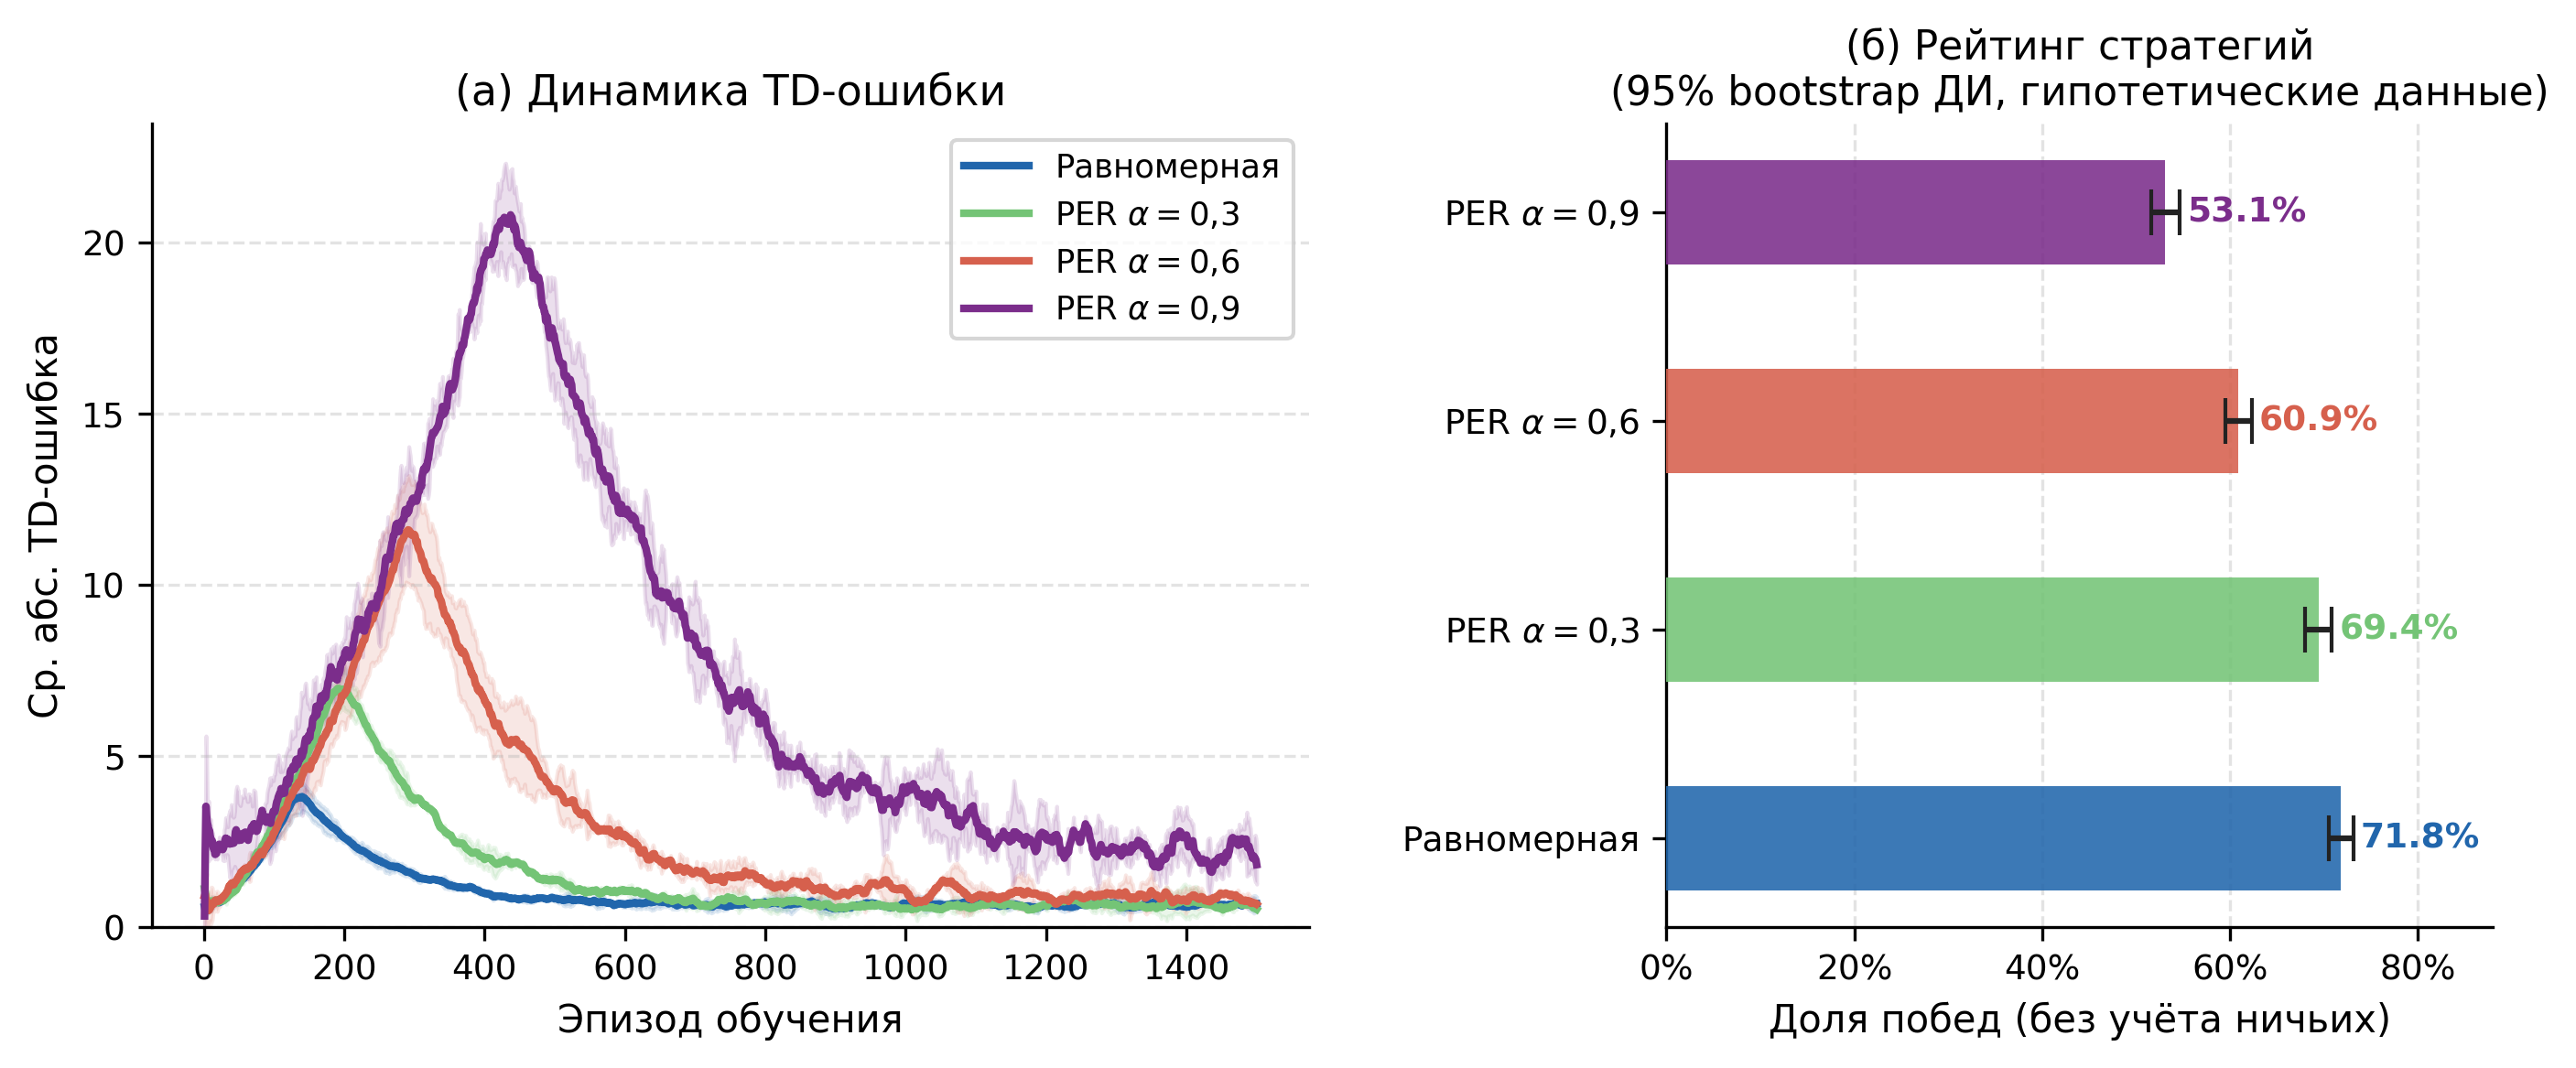
\includegraphics[width=\linewidth]{figures/fig_combined.png}
    \vspace{-4pt}
    {\color{pgray}\scriptsize
      (а) Динамика $|\delta|$ — при $\alpha{=}0{,}9$ пик ${\approx}21{,}4$.%
      \quad
      (б) Win rate с 95\% CI.}

    \column{0.42\textwidth}

    \vspace{0.3cm}
    \begin{tabular}{@{}ccr@{}}
      \toprule
      $\alpha$ & Win rate & 95\% CI\\
      \midrule
      \good{0}   & \good{71,8\%} & \muted{[70,5;\,73,1]}\\
      0,3        & 69,4\%        & \muted{[68,0;\,70,8]}\\
      0,6        & 60,9\%        & \muted{[59,5;\,62,3]}\\
      \bad{0,9}  & \bad{53,1\%}  & \muted{[51,6;\,54,6]}\\
      \bottomrule
    \end{tabular}

    \vspace{0.5cm}

    % Delta highlight
    \begin{tikzpicture}
      \node[fill=pblue!10,rounded corners=6pt,
            align=center,inner sep=10pt] {
        {\color{pblue}\bfseries$\Delta = +18{,}7$ п.п.}\\[3pt]
        {\small\color{pdark}$\alpha{=}0$ vs $\alpha{=}0{,}9$}\\
        {\small\color{pgray}95\% CI $\not\ni 0$}
      };
    \end{tikzpicture}

  \end{columns}

  \note{
    Главный слайд.

    Левый рисунок — динамика TD-ошибки. При alpha=0.9 ошибка нарастает
    до 21.4 к эпизоду 420, затем снижается, но не до уровня alpha=0.
    При alpha=0 — монотонное убывание до 3.8. Нестабильное обучение.

    Правый: таблица win rate. Монотонное убывание с ростом alpha.
    Разница крайних значений: 18.7 п.п., CI не содержит ноль.

    Отметим: alpha=0.3 vs alpha=0 — лишь 2.4 п.п., может быть в пределах
    вариативности между инициализациями.
  }
\end{frame}


%──────────────────────────────────────────────────────────────────────────────
% 8. BIG NUMBERS
%──────────────────────────────────────────────────────────────────────────────
\begin{frame}{}  % без заголовка — акцент на числах

  \vspace{0.6cm}
  \begin{center}

    {\color{pgray}\small Итоговый win rate по результативным партиям}

    \vspace{0.5cm}

    \begin{tikzpicture}[font=\normalsize]

      % alpha=0 box
      \node[fill=pgreen!15,rounded corners=10pt,
            minimum width=3.8cm,minimum height=3.2cm,
            align=center,inner sep=12pt] (n0) at (-5,0) {
        {\color{pgreen}\fontsize{42}{44}\selectfont\bfseries 71,8\%}\\[6pt]
        {\color{pgray}\small $\alpha = 0$}\\
        {\color{pgray}\scriptsize (равном. выборка)}
      };

      % arrow + delta
      \node[align=center] at (0,0) {
        {\color{pblue}\Large$\longrightarrow$}\\[4pt]
        {\color{pblue}\bfseries$-18{,}7$ п.п.}\\
        {\color{pgray}\scriptsize при росте $\alpha$}
      };

      % alpha=0.9 box
      \node[fill=psalmon!15,rounded corners=10pt,
            minimum width=3.8cm,minimum height=3.2cm,
            align=center,inner sep=12pt] (n9) at (5,0) {
        {\color{psalmon}\fontsize{42}{44}\selectfont\bfseries 53,1\%}\\[6pt]
        {\color{pgray}\small $\alpha = 0{,}9$}\\
        {\color{pgray}\scriptsize (макс. приоритет)}
      };

    \end{tikzpicture}

    \vspace{0.5cm}
    {\color{pgray}\small
      Тенденция монотонна; разностный bootstrap-ДИ не содержит нуль.}

  \end{center}

  \note{
    Этот слайд подчёркивает главный результат: разница почти 19 процентных
    пунктов между равномерной выборкой и максимальной приоритизацией.

    Равномерный DQN оказался лучше PER при всех ненулевых значениях alpha
    в данной постановке.
  }
\end{frame}


%──────────────────────────────────────────────────────────────────────────────
% 9. CONCLUSIONS
%──────────────────────────────────────────────────────────────────────────────
\begin{frame}{Выводы}

  \vspace{0.3cm}
  \begin{columns}[c]

    \column{0.52\textwidth}

    \begin{tikzpicture}[font=\small]
      \node[fill=pgreen!12,rounded corners=6pt,
            text width=5.8cm,inner sep=9pt] (a) {
        \good{\checkmark}\enspace
        Win rate \textbf{монотонно убывает} с ростом $\alpha$
      };
      \node[fill=pgreen!12,rounded corners=6pt,
            text width=5.8cm,inner sep=9pt,below=0.25 of a] (b) {
        \good{\checkmark}\enspace
        Разность $\alpha{=}0$ vs $\alpha{=}0{,}9$:
        \hilight{$+18{,}7$ п.п.}
      };
      \node[fill=pgreen!12,rounded corners=6pt,
            text width=5.8cm,inner sep=9pt,below=0.25 of b] (c) {
        \good{\checkmark}\enspace
        Высокий $\alpha$ → пиковые $|\delta|$ и нестабильное обучение
      };
      \node[fill=pblue!10,rounded corners=6pt,
            text width=5.8cm,inner sep=9pt,below=0.25 of c] (d) {
        \hilight{\bfseries Вывод:} равномерная выборка ($\alpha{=}0$)
        оказалась оптимальной при данном бюджете и setup-е
      };
    \end{tikzpicture}

    \column{0.44\textwidth}

    \textbf{Ограничения:}
    \begin{itemize}\setlength\itemsep{4pt}
      \item Bootstrap-ДИ по партиям, не по seeds
      \item $\beta$-schedule не оптимизировался совместно с $\alpha$
      \item Draw rate 57–74\% влияет на метрику
    \end{itemize}

    \vspace{0.4cm}
    \textbf{Перспективы:}
    \begin{itemize}\setlength\itemsep{4pt}
      \item Адаптивный $\alpha$ по динамике $|\delta|$
      \item Совместный подбор $\alpha$ и $\beta$
      \item Больший бюджет ($\geq\!5\,000$ эп., $n\geq\!10$)
    \end{itemize}

  \end{columns}

  \note{
    Три ключевых вывода:
    1. Монотонное убывание при росте alpha.
    2. Разница 18.7 п.п. — статистически значима по партиям.
    3. Нестабильность обучения при высоком alpha.

    Важная оговорка: мы не говорим, что PER плох в принципе.
    Возможно, совместная оптимизация alpha и beta даст другой результат.
    Практический вывод: не переносить alpha=0.6 из Atari вслепую.

    Перспективы: адаптивный alpha, который снижается при нестабильности.
  }
\end{frame}


%──────────────────────────────────────────────────────────────────────────────
% 10. THANKS
%──────────────────────────────────────────────────────────────────────────────
\begin{frame}[plain]

  {\color{pblue!40}\rule{\paperwidth}{2pt}}\vspace{-2pt}

  \vspace{1.6cm}
  \begin{center}

    {\color{pdark}\LARGE\bfseries Спасибо за внимание!}

    \vspace{0.8cm}

    \begin{tikzpicture}
      \node[fill=plbg,rounded corners=8pt,
            align=center,inner sep=14pt,minimum width=9cm] {
        {\color{pblue}\bfseries Агрессивная приоритизация дестабилизирует self-play.}\\[6pt]
        {\color{pgray}\small $\alpha{=}0$: \good{71,8\%} \quad vs \quad $\alpha{=}0{,}9$: \bad{53,1\%}}\\[3pt]
        {\color{pgray}\small Равномерная выборка победила в данной постановке.}
      };
    \end{tikzpicture}

    \vspace{0.6cm}
    {\color{pgray}
      М.\,А. Самойлов \quad\texttt{samoilov\_m1@yandex.ru}}

    \vspace{0.4cm}
    {\color{pgray}\small Вопросы?}

  \end{center}

  \vfill
  {\color{pblue!30}\rule{\paperwidth}{1pt}}

  \note{
    Готов ответить на вопросы.

    Частые вопросы:
    - Архитектура: 2 Conv + 2 Linear, 4096 Q-выходов.
    - Почему ничьи исключены: их 57-74%, они заглушают сигнал.
    - Negamax: в zero-sum V(s) = -V_opp(s'), это важно для корректного таргета.
    - Imitation warm-start: поведенческое клонирование от HeuristicAgent.
    - Bootstrap CI: 10000 ресэмплов по партиям, не по seeds.
  }
\end{frame}


\end{document}
